%%%%%%%%%%%%%%%%%%%%%%%%%%%%%%%%%%%%%%%%%%%%%%%%%%%%%%%%%%%
% EPFL report package, main thesis file
% Goal: provide formatting for theses and project reports
% Author: Mathias Payer <mathias.payer@epfl.ch>
%
% To avoid any implication, this template is released into the
% public domain / CC0, whatever is most convenient for the author
% using this template.
%
%%%%%%%%%%%%%%%%%%%%%%%%%%%%%%%%%%%%%%%%%%%%%%%%%%%%%%%%%%%
\documentclass[a4paper,11pt,oneside]{report}
% Options: MScThesis, BScThesis, MScProject, BScProject
\usepackage[BScThesis,lablogo]{EPFLreport}
\usepackage{xspace}
\usepackage{xcolor}
\usepackage{listofitems}
\usepackage{subcaption}

\newif\ifreview
\reviewtrue
% To remove the reviews seet \reviewfalse
%\reviewfalse

\definecolor{amber}{rgb}{1.0, 0.75, 0.0}
\newcounter{ReviewerID}
\readlist*\annotationcolors{blue, red, orange, green, purple, amber, brown, olive}
\newcommand{\newreviewer}[2]{%
	\ifnum \theReviewerID=\annotationcolorslen
	\setcounter{ReviewerID}{0} % cycle through colors
	\fi
	\stepcounter{ReviewerID}%
	\expandafter\edef\csname bootstrap#1\endcsname{%
		\expandafter\def\csname #1\endcsname####1{%
			\ifreview%
			 {\noexpand\color{\annotationcolors[\theReviewerID]} {\noexpand\bf{\noexpand\fbox{#2}} {\noexpand\it ####1} }}
			\else%
			 {}% disable annotations
			\fi%
		}%
	}%
	\csname bootstrap#1\endcsname%
}

\newreviewer{philipp}{philipp}

\title{Tooling and Analysis of the Scudo Allocator}
\author{Elias Valentin Boschung}
\supervisor{Mao Philipp Yuxiang}
\adviser{Prof. Dr. sc. ETH Mathias Payer}
%\coadviser{Second Adviser}
%\expert{The External Reviewer}

\newcommand{\sysname}{Scudo GEF Plugin\xspace}

\begin{document}
\maketitle{}
\dedication{
  \begin{raggedleft}
    If debugging is the process of removing software bugs,\\
    then programming must be the process of putting them in.\\
    --- Edsger Dijkstra\\
  \end{raggedleft}
  \vspace{4cm}
  \begin{center}
    Dedicated to my study companion since Covid-19, my plush bear.
  \end{center}
}
\makededication{}
\acknowledgments{
I thank first and foremost my family for their unconditional
support throughout all of my studies until this point. I also thank my
supervisor Philipp for all the tips and the help in writing this project.
Thanks to my friends, those who inspired and encouraged me on the path of
cybersecurity, as well as those who helped me relax when I was stressed.
Thanks also to the HexHive lab for the opportunity to do this Bachelor
Project, and also for providing the template for this report, which is
available at \url{https://github.com/hexhive/thesis_template}.}
\makeacks{}

\begin{abstract}
Heap related memory corruptions are a major concern.
To understand the cause and impact of such heap bugs,
developers and analysts rely on tools that allow them to
dynamically inspect the state of the heap.
LLVM's Scudo heap implementation is a hardened memory allocator that 
attempts to prevent exploitation of common heap related bugs.
Since Android 11, Scudo is used as the main memory allocator for Android apps.
Due to its novelty only little documentation exists on how Scudo 
works internally, and no tooling exists to inspect the state of the Scudo heap.
In this project we analyse the way Scudo manages the heap and
develop a tool to analyse the state of the Scudo heap at runtime.
We implement our tool as an extras plugin into the popular GEF plugin for GDB.
We demonstrate that we can leverage our tool to triage heap related bugs in 
Android native libraries running on Android 11 (Security patch level 1 January 2021).

\end{abstract}

\maketoc{}

%%%%%%%%%%%%%%%%%%%%%%
\chapter{Introduction}
%%%%%%%%%%%%%%%%%%%%%%

Bugs related to heap memory are one of the most frequent problems encountered
by C developers, since in bigger projects it can very quickly get hard to track
all the resources that are open and which were already closed. It is very tedious
to track all of such errors down, and just a single oversight might create a bug
that opens a huge security vulnerability. Additionally, nowadays, many apps are so
complex that they use various third-party libraries to do different tasks, since
re-implementing everything on your own would be a waste of time. However, one
hardly has the time to check the whole source code of every library one uses, so
one has to trust the library developers to have done their work correctly. An
example of where such trust was the cause of a major vulnerability is a remote
code execution in WhatsApp that was found in 2019, where a simple double free
in a third-party GIF library allowed an attacker to get arbitrary remote code
execution.~\cite{whatsappRCE}

Since checking all the code of all third-party libraries is practically not
feasible, it is important to be able to debug heap bugs when they are found, in
order to understand how they happen, the consequences an exploit using the
bug might have, and to be able to fix the bug rapidly. In order to encourage
and assist developers in this process, there needs to be some freely available
tools that make dynamic debugging of the heap easier.

Since Android devices are used daily by millions of users, with many thousands to
millions of different apps, the attack surface for exploits is huge. That might
well be one of the reasons that Android uses the new and mostly unknown heap
allocator called Scudo.~\cite{llvmScudo} Scudo tries to mitigate some of the potential
vulnerabilities due to heap bugs directly in the allocator, while keeping a high
performance for memory allocations. However, since it is relatively new, there
exists only spare documentation of how Scudo functions internally, and there
are no tools to dynamically analyze the Scudo heap.

The \textit{Androlib} project is an ongoing 
project at the HexHive lab to fuzz Android native libraries.
As a result of fuzzing campaigns carried out, \textit{Androlib} has discovered a 
number of crashes in native libraries.
While it is doable to triage the crashes in some categories, heap-related
crashes are difficult to analyse due to the Scudo allocator, as no tooling 
to inspect the Scudo heap exists.

The goal of this project is therefore to implement a tool that allows to dynamically 
inspect the Scudo heap. 
One of the main challenges is 
to understand the Scudo allocator internals and then to
create appropriate tooling to help with the analysing of those crashes.
While there is a bit of documentation around Scudo, there is not really a
comprehensive overview of all detailed inner workings of Scudo, and no 
tools tailored for debugging crashes related to Scudo.

Since \textit{Androlib} uses gdb and gef for it's triaging setup, we implement our tool as a gef-extras plugin, 
that can be easily loaded into gdb with gef and adds some commands for inspecting the
Scudo heap.
 
We evaluate our tool by triaging seven heap-related crashes on a real Android 
device.
We plan to open source our tool to make it available to the community.

%%%%%%%%%%%%%%%%
\chapter{Scudo Internals}
%%%%%%%%%%%%%%%%

The Scudo hardened allocator divides the heap allocations it is asked to do into
two big types of allocations, based on the size of the chunk to be allocated.
The smaller chunks are handled by the primary allocator inside Scudo, which is
designed to optimize performance as much as possible by adapting to finer grained
size differences between these smaller chunks. All the big chunks are handled by
the secondary allocator, which is less optimized, since the most frequent chunks
are the small ones and thus the primary allocator has a bigger impact on performance
than the secondary allocator.

\section{Chunk Header}

\begin{figure}[h]
  \centering
  \begin{tabular}{lr}
    ClassId           & 8 bits  \\
    State             & 2 bits  \\
    OriginOrWasZeroed & 2 bits  \\
    SizeOrUnusedBytes & 20 bits \\
    Offset            & 16 bits \\
    Checksum          & 16 bits
  \end{tabular}
  \caption{Layout of the Scudo chunk header}
  \label{fig:ScudoChunkHeader}
\end{figure}

The chunks allocated by both the primary and the secondary allocator store some
metadata in a combined header. This header is then stored just in front of the
actual content of the chunk, such that it can easily be checked whenever the
chunk gets accessed. An overview of the contents of this header can be seen
in \autoref{fig:ScudoChunkHeader}. The ClassId identifies the class the chunk
belongs to in case it was allocated by the primary allocator, with a ClassId
of 0 meaning that the chunk was allocated by the secondary allocator. The
header also contains information about the state of the chunk, which can be
allocated, quarantined or available, as well as the origin of the allocation,
e.g., malloc or new, which can be used to detect errors when the type of
deallocation does not match the type of the allocation. Furthermore, the
header includes the size for the primary chunks or the amount of unused bytes
for the secondary chunks and an offset, which is the distance from the beginning
of the returned chunk to the beginning of the actual backend allocation.
Finally, the header contains a checksum, which is generated using a cookie (a
random number generated during the initialization of the allocator), the heap
address of the chunk, and the actual content of the header. This checksum is
used for guarding against programming errors as well as attackers, and it is
checked each time the header is loaded.

\section{Primary Allocator}

The primary allocator structures the heap into Classes (also named Regions), the
amount of which depend on the configuration. These classes are identified by a
ClassId, starting from 1. The ClassId 0 is reserved for allocating the internal
structures used by Scudo to keep track of the free chunks.
Each of the classes gets its own region in memory where it can allocate chunks,
giving some separation between chunks of different classes, unlike the standard
libc heap allocator, where the heap is a single big region in memory. This can
also be seen in \autoref{fig:ScudoPrimaryRegionsOverview}, where we see that
each class/region has its own beginning address, and also tracks its own mapped
and allocated space.

\begin{figure}[h!]
  \centering
  \includegraphics[width=\linewidth]{figures/ScudoPrimaryRegionsOverview.png}
  \caption{Example of the division of classes/regions by using the developed plugin}
  \label{fig:ScudoPrimaryRegionsOverview}
\end{figure}


The classes have a given size of the chunks that can be allocated in that class,
which increases with the ClassId, with the exact numbers depending again on the
configuration. An excerpt of the class sizes on Android 11 can be seen in
\autoref{fig:ScudoAndroidClasses}.

\begin{figure}[h!]
  \centering
  \begin{tabular}{lr}
    \textbf{ClassId} & \textbf{Size of chunks} \\
    0                & special                 \\
    1                & 0x20                    \\
    2                & 0x30                    \\
    3                & 0x40                    \\
    4                & 0x50                    \\
    ...              & ...                     \\
    36               & 0x30010                 \\
    37               & 0x38010                 \\
    38               & 0x40010                
  \end{tabular}
  \caption{Sizes of the classes on Android 11}
  \label{fig:ScudoAndroidClasses}
\end{figure}

So the chunk that is actually returned by the primary allocator might be bigger
than what was asked for, but this helps against having to do expensive bookkeeping
to avoid fragmentation inside the classes.

So when an allocation request is made to Scudo, and it is small enough to fit into
one of the primary allocator regions, then the primary allocator first finds the
smallest class that still contains chunks big enough for the requested size. It
then checks in the cache associated to that class, to find a chunk that is already
available. However, if the cache is empty, meaning that there are no readily
available free chunks, the primary allocator tries to refill the cache with some
new chunks. For that purpose, it looks up the freelist of TransferBatches for the
given class, and if it is not empty it just takes all the chunks of the first
TransferBatch in the freelist and moves them to the cache of the class. One
TransferBatch holds a certain number of chunks defined by the configuration,
which is the same for all classes.
In case the freelist is out of TransferBatches, the allocator will allocate
some new TransferBatches to fill up the freelist. The amount of TransferBatches
allocated at one such time depends on the configuration, but it is typically
smaller the bigger the class gets, as one TransferBatch represents more actual
memory the bigger the class is. The allocator will also map more space for a
specific class if the amount of TransferBatches to be created does not fit into
the existing mapped space.
Since the transfer batches that are currently in one of the freelists need to
be stored somewhere as well, the first class with ClassId 0 is reserved for
this use. The allocations requested by the user will never directly use this
class, instead when a freelist for one of the classes needs to be refilled
with new TransferBatches, these are allocated in this first class, and they
are freed when they are moved to the cache of the class.

\begin{figure}[h!]
  \centering
  \begin{subfigure}{.5\textwidth}
    \centering
    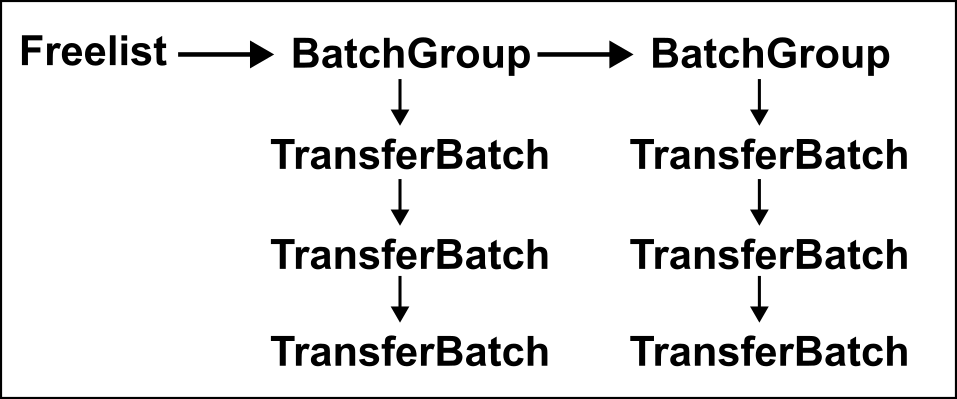
\includegraphics[width=.9\linewidth]{figures/ScudoPrimaryFreelistLatest.png}
    \caption{Latest version}
    \label{fig:ScudoPrimaryFreelistLatest}
  \end{subfigure}%
  \begin{subfigure}{.5\textwidth}
    \centering
    
\includegraphics[width=.9\linewidth]{figures/ScudoPrimaryFreelistAndroid.png}
    \caption{Version shipped with Android 11}
    \label{fig:ScudoPrimaryFreelistAndroid}
  \end{subfigure}
  \caption{Layout of the freelist for each of the classes}
  \label{fig:ScudoPrimaryFreelist}
\end{figure}

Additionally, while not yet present in the version of Scudo shipped with Android
11, the latest Scudo version includes a type that regroups multiple transfer
batches, into a BatchGroup, as illustrated in \autoref{fig:ScudoPrimaryFreelistLatest}.
Instead of the freelist for a given class containing
a list of transfer batches, it now has a list of batch groups, which contain
a list of transfer batches each. The overall functionality of the allocator
doesn't change however, the change is just supposed to get even more performance
for the frequent allocations of the primary allocator.

\section{Secondary Allocator}

The secondary allocator is a bit less sophisticated, since it does not need to
be able to do as many allocations and deallocations as the primary allocator,
and the optimizations of the primary allocator would not be that efficient for
the bigger and therefore generally more variable sizes the secondary allocator
has to handle. Instead, the secondary allocator just keeps a simple cache of
the previously freed chunks, and if there is no matching chunk in its cache
upon a request for a new allocation, it maps some new memory for that chunk.
For bookkeeping, the secondary allocator simply keeps a doubly linked list of
all chunks currently in use and keeps track of the details of each allocated
chunk in a special header that is prepended to the combined header.

%%%%%%%%%%%%%%%%%%%%%%%%
\chapter{Implementation}
%%%%%%%%%%%%%%%%%%%%%%%%

The structure of the gef-extras plugin is heavily inspired by the existing
structure of the tooling for the standard libc heap allocator used in most
Linux systems, which is included in the gef plugin for gdb.~\cite{gef} The
Scudo plugin therefore offers multiple commands for the different structures
present in Scudo. These commands take generally some address to a memory
region, and create an object by reading out the data from that memory address
and parsing it according to the predefined structure.

The most basic command is the \verb|scudo chunk| command, which given the address
of a chunk on the heap, reads the header in front of the chunk and displays
the info contained in it. The design of the output is the same as for the
standard libc heap commands included in gef, with the allocation state being
highlighted in color, as can be seen in \autoref{fig:ScudoChunkCommand}.
In the actual implementation, a chunk is represented as a class, and like in
gef, the different information is stored as properties of the class. Similarly,
the data is read from memory using the \verb|gef.memory.read| function, and then
structured as a type using the ctypes library to represent the different types
used in Scudo. The \verb|str| method on the class is implemented to display a short
summary of the most essential info, while the \verb|psprint| method shows the
extended information display, as shown in \autoref{fig:ScudoChunkCommand}.

\begin{figure}[h!]
  \centering
  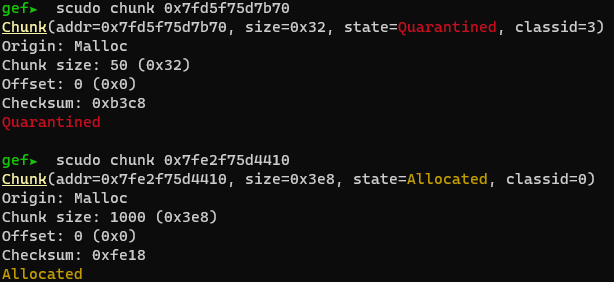
\includegraphics[width=\linewidth]{figures/ScudoChunkCommand.png}
  \caption{Example of the Scudo chunk command in gef}
  \label{fig:ScudoChunkCommand}
\end{figure}

The next two commands concern the region info, with respectively the
\verb|scudo region| and \verb|scudo regions| commands. Both of work with the same
\verb|ScudoRegionInfo| class, which is defined like the Scudo chunk with a ctypes
structure to represent the types in the Scudo c code, and with properties for
all the information extracted. The one special thing about the region info
class is the padding, since the structure is padded to the Scudo cache line
size for faster access. So the plugin first builds an unpadded version of the
ctypes structure, and then adds the required padding to get a multiple of the
Scudo cache line size to the structure to get the final version.

The info included in the RegionInfo structure includes the list of transfer
batches for that region, the number of popped and pushed blocks, the amount
of memory mapped and allocated inside the region, the random state generated
for the region as well as information about the last release of blocks to
the operating system.

The data of this \verb|RegionInfo| structure is stored in an array, with an entry
for each of the regions/classes. The array is part of the primary allocator
class, and so the plugin finds it by using the offset from the \verb|Allocator|
symbol to get the first entry in the array.
The \verb|scudo regions| command then simply displays a list of short information
about each region, as seen in \autoref{fig:ScudoRegionsCommand}.

\begin{figure}[h!]
  \centering
  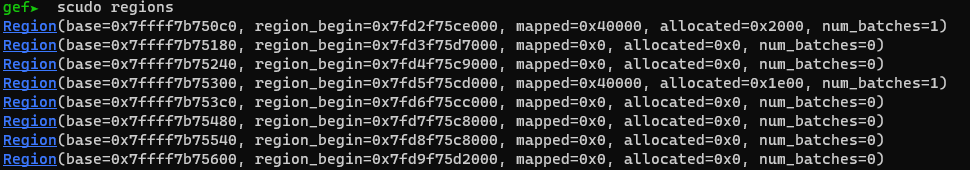
\includegraphics[width=\linewidth]{figures/ScudoRegionsCommand.png}
  \caption{Example of the Scudo regions command in gef}
  \label{fig:ScudoRegionsCommand}
\end{figure}

The \verb|scudo region| command on the other hand displays more detailed information
about a specific region, which can be specified either by giving the address
to the RegionInfo structure, by giving the max allocation size of the region,
or by the index in the array, which corresponds to its ClassId. An example of
the display can be seen in \autoref{fig:ScudoRegionCommand}, which shows the
special region which holds the transfer batches.

\begin{figure}[h!]
  \centering
  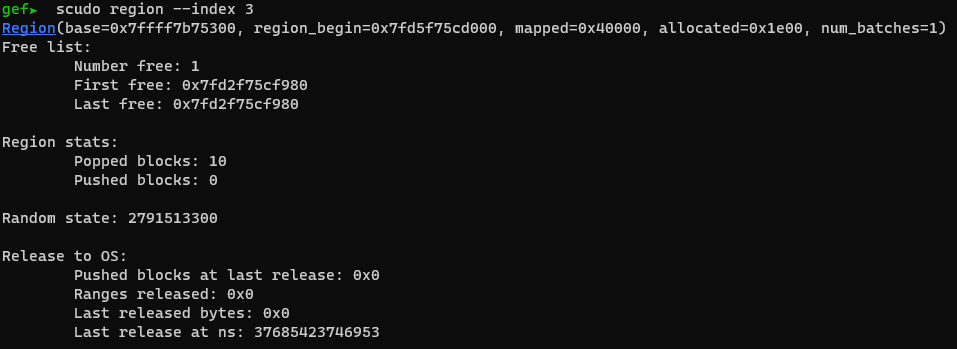
\includegraphics[width=\linewidth]{figures/ScudoRegionCommand.png}
  \caption{Example of the Scudo region command in gef}
  \label{fig:ScudoRegionCommand}
\end{figure}

The next two commands concern the free list of the primary allocator, as they
display the information about the batch groups and the transfer batches. Both
of these commands are very simple, since both of them basically contain a list
of another structure. Also since there isn't one universal point where all of
them are stored, the commands need to be provided with the address of the
batch group or transfer batch to output.
Since the batch groups are a new addition, the command doesn't work on a real
Android 11 phone, however it works when using the standalone compiled version
from the llvm repository. It shows detailed information about the batch group,
including the address of the next batch group, since the batch groups form a
linked list, the number of pushed blocks, and the information about the doubly
linked list of transfer batches it contains. While this detailed view can be
seen in \autoref{fig:ScudoBatchGroupCommand}, when specifying a number as
argument with \verb|--number X|, it will instead display a short version for this
amount of batch groups in the linked list, with the first one being the one
specified by address.

\begin{figure}[h!]
  \centering
  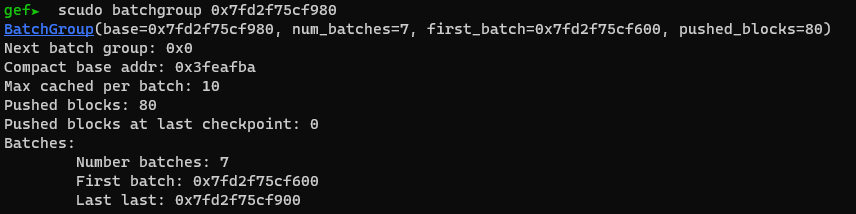
\includegraphics[width=\linewidth]{figures/ScudoBatchGroupCommand.png}
  \caption{Example of the Scudo batch group command in gef}
  \label{fig:ScudoBatchGroupCommand}
\end{figure}

The \verb|scudo transferbatch| command simply outputs the addresses of every batch
it contains, as well the address of the next transfer batch, which can be seen
in \autoref{fig:ScudoTransferBatchCommand}. Since the transfer batches also
form a linked list similarly to the batch groups, the number argument can be
specified in the same way to get an overview of that number of transfer batches.

\begin{figure}[h!]
  \centering
  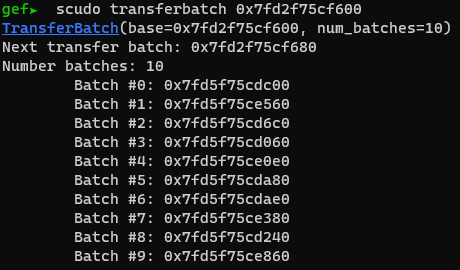
\includegraphics{figures/ScudoTransferBatchCommand.png}
  \caption{Example of the Scudo transfer batch command in gef}
  \label{fig:ScudoTransferBatchCommand}
\end{figure}

The next command concerns the cache, which is actually the first place the
primary allocator tries to look for free chunks to allocate for the user.
While again the content of each per class structure is fairly simple with a
list of the chunks it contains and the maximal number of chunks it can contain,
there was a particular challenge about implementing this command, which was to
find the location of the actual array. Since Scudo was designed for multi
threading, there actually exists a cache for each thread, and as such the per
class array of each thread is not simply stored at an offset from the Allocator
symbol. However, there luckily is a trick to find the different per class arrays
of the different threads, as the cache of each thread contains some statistics
about the allocated and free blocks in that cache. In order to have some global
statistics over all the different threads, Scudo stores some global stats, that
include a linked list of all the local stats of the different threads. So in
order to get the address of the per class array of a thread, the plugin gets
the linked list of statistics from its offset to the Allocator symbol and then
follows the linked list the number of times to reach the statistics for the
correct thread. Since the statistics are stored right after the per class array
in the cache, the plugin then simply subtracts the size of the per class array
to get the address of the first entry in the class array.
For that reason the \verb|scudo perclass| command also takes two arguments, the first
being the thread ID and the second being the class ID, which uniquely define
the entry to get. If the IDs are omitted a default value of 0 is taken. An
example of the output can be seen in \autoref{fig:ScudoPerClassCommand}.

\begin{figure}[h!]
  \centering
  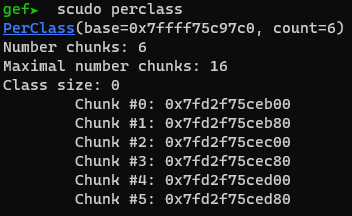
\includegraphics{figures/ScudoPerClassCommand.png}
  \caption{Example of the Scudo per class command in gef}
  \label{fig:ScudoPerClassCommand}
\end{figure}

The last command is the only one concerning the secondary allocator specifically,
and it reads out the special header that is prepended to the normal chunk header
for any secondary chunk. The normal Scudo chunk command still works for secondary
chunks as well though. The large block command gives information about the
commit and map base addresses and sizes, as well as the next and previous large
blocks in the linked list. The command can either be provided by an address
to read out the corresponding large block, or if the address is omitted it will
take the first block from the list of blocks in use. An example can be seen in
\autoref{fig:ScudoLargeBlockCommand}. A \verb|--number X| argument can optionally be
specified to get once again a list of short information about that amount of large
blocks.

\begin{figure}[h!]
  \centering
  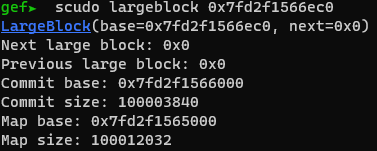
\includegraphics{figures/ScudoLargeBlockCommand.png}
  \caption{Example of the Scudo large block command in gef}
  \label{fig:ScudoLargeBlockCommand}
\end{figure}

While the whole plugin is contained in a single file to follow the gef standard,
the organization with classes and using the ctypes structures allows for a
flexibility in adapting and evolving the plugin. As such it would be quite
easy to adapt the plugin for any minor changes in the Scudo structure should
it evolve in the future, or adapted to support older versions of Scudo, with
one such version already being implemented for the version of Scudo that was
shipped with Android 11. The main changes for this older version of Scudo
included that the batch groups did not exist yet, some minor reordering of
some fields in some of the structures, which also caused some of the offsets
from the Allocator symbol to be changed.


%%%%%%%%%%%%%%%%%%%%
\chapter{Evaluation}
%%%%%%%%%%%%%%%%%%%%

To evaluate our tool, we first want to show that we can install and use the
tool on a real android phone, and then that it can help with investigating
crashes taken from real android apps using native libraries.

\section{Setup on real Android phone}

During the main development process the plugin was tested with the standalone
version of Scudo compiled with debug symbols from the llvm repository. In
order to get the plugin loaded by gef, the folder containing the plugin file
needs to be specified as gef-extras plugin directory. The easiest way to do this
is to run \verb|gef config gef.extra_plugins_dir /path/to/plugin/dir|. In order
to use multiple different gef extra plugins that may be located at different
paths, multiple paths can be specified separated by semicolons. Also, the
configuration can be saved using \verb|gef save|, which will create a gef.rc file
that will be loaded in order to keep the settings between restarts of gdb.

Since the main development was done on the standalone version, the first step
to evaluate the plugin was to actually test it on a real android phone. The
test device was a Samsung Galaxy S10, which was already rooted using Magisk
and had gdb and gef installed using the Termux app. Access to the phones
console and copying of the plugin to the phone was done using adb.

While the plugin installation and loading worked without problem on the phone, it
rapidly became evident that the plugin did not work as intended and instead
returned some random looking numbers for most commands. So after some
investigation, it was discovered that the Scudo version shipped with Android
11, which was installed on the testing device, differed in multiple points
from the most recent version on the llvm repository. The plugin was therefore
copied and adapted into a version for Android 11, which notably does not
contain the batch groups, as well as differing in some minor changes in
different structures.

\section{Crash Triage}

\subsection{Overview}
In order to evaluate the actual functioning of the plugin, it was tested with
some of the crashes found in the \textit{Androlib} fuzzing campaign. 
The starting of the corresponding apps and causing the crashes was already
set up automatically, including opening gdb before starting to run the program
in order to allow for the setting of any breakpoints if needed. In
\autoref{fig:ScudoTriageOverview} we can see an overview of the crashes analyzed.
We will show two detailed case studies and how the plugin and some specific
commands helped in analyzing them in the next section.

\begin{figure}[h!]
  \centering
  \begin{tabular}{lll}
    \textbf{Package name}                     & \textbf{Crash \# from Androlib} & \textbf{Crash reason} \\
    com.skt.smartbill                         & BT5                             & invalid free           \\
    & BT7                             & double free           \\
    & BT13                            & double free           \\
    heartratemonitor.heartrate.pulse.pulseapp & BT1                             & header corruption     \\
    com.ahnlab.v3mobileplus                   & BT1                             & double free           \\
    com.kbankwith.smartbank                   & BT2                             & double free           \\
    & BT3                             & invalid free         
\end{tabular}
  \caption{Overview of the crashes triaged}
  \label{fig:ScudoTriageOverview}
\end{figure}

\subsection{Case studies}

\subsubsection{V3MobilePlus Backtrace 1}

The next crashed analysed is part of \verb|com.ahnlab.v3mobileplus| app,
numbered backtrace 1 in \textit{Androlib}. Again the first step was to find
the line in the library right before the crash happened, in order to be able
to investigate before the crash. So we set a breakpoint at \verb|BIN_Free+28|,
and after continuing over the breakpoint three times we are right before the
call to \verb|free| that causes the crash.

\begin{figure}[h!]
  \centering
  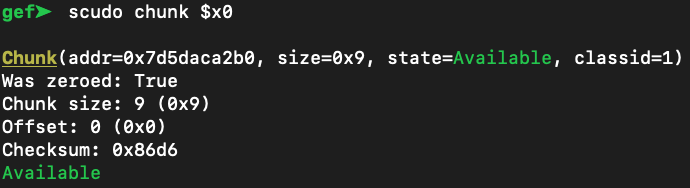
\includegraphics[width=\linewidth]{figures/ScudoV3MobilePlusOffendingChunk.png}
  \caption{Chunk header that causes a crash when freed}
  \label{fig:ScudoV3MobilePlusOffendingChunk}
\end{figure}

First we check the most simple thing, the header of the chunk that is about
to be freed. As can be seen in \autoref{fig:ScudoV3MobilePlusOffendingChunk},
there seems to indeed be a problem with the chunk, since it is already marked
as available, but the program wants to free it. So either it tries to free a
chunk it has already freed, or it tries to free a chunk it actually never
allocated. In order to investigate a bit further, we can check the first place
the chunk would have been put if it was previously allocated and freed, in the
cache's PerClass. Since the chunk has only a size of 9, we know it resides in
the first class, with ClassId 1. The output of checking this PerClass info can
be seen in \autoref{fig:ScudoV3MobilePlusPerClassAfter}.

\begin{figure}[h!]
\centering
\begin{minipage}{.5\textwidth}
  \centering
  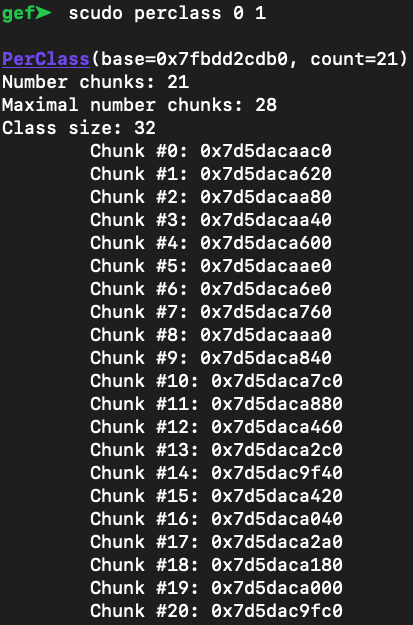
\includegraphics[width=.95\linewidth]{figures/ScudoV3MobilePlusPerClassAfter.png}
  \captionof{figure}{PerClass right before the crash}
  \label{fig:ScudoV3MobilePlusPerClassAfter}
\end{minipage}%
\begin{minipage}{.5\textwidth}
  \centering
  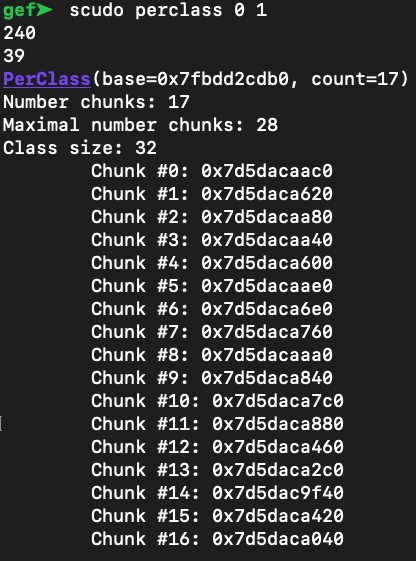
\includegraphics[width=.95\linewidth]{figures/ScudoV3MobilePlusPerClassBefore.png}
  \captionof{figure}{PerClass at the first break}
  \label{fig:ScudoV3MobilePlusPerClassBefore}
\end{minipage}
\end{figure}

With this output, we can check if the chunk at address \verb|0x7d5daca2b0| is
present in the cache, and indeed we see the address \verb|0x7d5daca2a0|, which
corresponds to the address of that chunk including the header. Since it is
present towards the end of the list of chunks in the cache, this is most likely
the case of a double free, where the chunk was already freed earlier in the app.
Indeed, by running through the crash again, we can see that at the first break at
\verb|BIN_Free+28|, the cache doesn't contain the offending chunk yet, as can be
seen in \autoref{fig:ScudoV3MobilePlusPerClassBefore}. Also by actually looking
at the chunk that is to be freed at this first break (\autoref{fig:ScudoV3MobilePlusChunkBefore}),
we see that it is the same chunk we try to free again later, resulting in the
program crashing as it tries to free the same chunk twice.

\begin{figure}[h!]
  \centering
  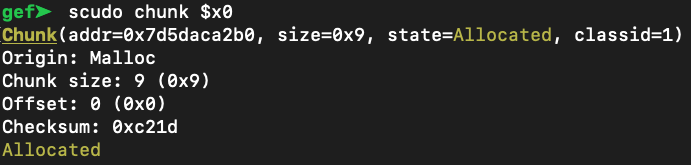
\includegraphics[width=\linewidth]{figures/ScudoV3MobilePlusChunkBefore.png}
  \caption{State of the chunk at the first break}
  \label{fig:ScudoV3MobilePlusChunkBefore}
\end{figure}

\subsubsection{Smartbill Backtrace 13}

This is another crash from the same app as the first crash we analysed. As we
once again first check the backtrace, we see that the functions right before the
crash are not named functions, so to break at the right point we take the offset
from the nearest named function, giving us a break at \verb|Convert_ASN1_to_X509_TBS_CERT+268-0xfdc|.

\begin{figure}[h!]
  \centering
  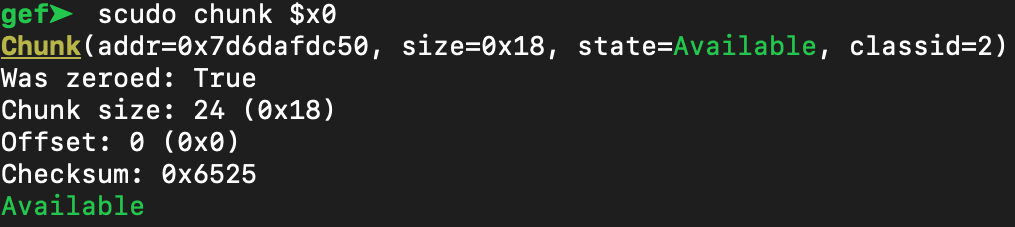
\includegraphics[width=\linewidth]{figures/ScudoSmartbillBT13OffendingChunk.png}
  \caption{State of the chunk at the break}
  \label{fig:ScudoSmartbillBT13OffendingChunk}
\end{figure}

As we can see in \autoref{fig:ScudoSmartbillBT13OffendingChunk}, we once again
try to free an already available chunk. So of course the next thing to verify
is again the cache of the corresponding class. The chunk command told us that
its ClassId is 2, so we check the main thread cache for this class, and as we
can see in \autoref{fig:ScudoSmartbillBT13PerClassAfter}, the chunk is indeed
in the cache at the last position, so we face most likely a double free bug
again.

\begin{figure}[h!]
  \centering
  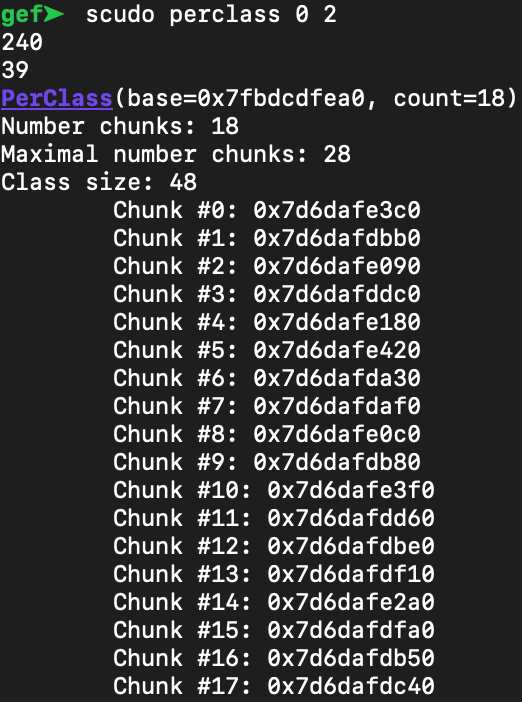
\includegraphics[width=.5\linewidth]{figures/ScudoSmartbillBT13PerClassAfter.png}
  \caption{PerClass of the main thread at the break}
  \label{fig:ScudoSmartbillBT13PerClassAfter}
\end{figure}



%%%%%%%%%%%%%%%%%%%%
\chapter{Conclusion}
%%%%%%%%%%%%%%%%%%%%

In this project we implemented a plugin for GDB/GEF to help analyse and debug
heap related crashes dynamically when the Scudo allocator is used as heap allocator.
The plugin works on real Android phones as well as on the standalone Scudo
version, and it can easily be loaded inside gef. The commands of the plugin
allow the inspection of the most important structures of Scudo, which can
be used in investigating real crashes. While the source code of Scudo was
already openly accessible and there was some documentation about Scudo, there
was no easy way to investigate crashes related to Scudo dynamically and directly
on a real phone for real Android apps with native libraries. While the plugin
handles the most important structures, it also builds a base which could be
extended to analyse further structures used by Scudo, like quarantine related ones.

\cleardoublepage{}
\phantomsection{}
\addcontentsline{toc}{chapter}{Bibliography}
\printbibliography{}

\end{document}
